\documentclass{ximera}

\title{Higher Order Derivatives Activity Solution Guide}
\author{MATH 425: Calculus I}

\begin{document}
\begin{abstract}
    Working with the peers in your group, solve the following problems. Make sure to show and justify all your work. Make sure everyone in the group understands the solution and participates. Be prepared to report your answers to the whole class. 
\end{abstract}
\maketitle


\begin{exercise}
    Calculate $f^{(k)}(x)$ for $0<k\leq 5$ where $f(x)=x^4+ax^3+bx^2+cx+d$, where $a,b,c,d$ are constants.\\
    \textcolor{blue}{ $f(x)=x^4+ax^3+bx^2+cx+d$ (for $k=0$, the zeroth derviatve, we just have the function)\\
    $f'(x)=4x^3+3ax^2+2bx+c$\\
    $f''(x)=12x^2+6ax+2b$\\
    $f'''(x)=24x+6a$\\
    $f^{(4)}(x)=24$\\
    $f^{(5)}(x)=0$}
\end{exercise}


\begin{exercise}
    Calculate the first five derivatives of $f(x)=\sqrt{x}$.  Use your derivatives to answer the following questions.\\
    \textcolor{blue}{$f'(x)=\frac{1}{2}x^{-\frac12}$\\
    $f''(x)=-\frac{1}{4}x^{-\frac{3}{2}}$\\
    $f'''(x)=\frac38x^{-\frac{5}{2}}$\\
    $f^{(4)}(x)=-\frac{15}{16}x^{-\frac{7}{2}}$\\
    $f^{(5)(x)}=\frac{105}{32}x^{-\frac{9}{2}}$}
        \begin{enumerate}
            \item Show that $f^{(n)}(x)$ is a multiple of $x^{-n+\frac12}$.\\
            \textcolor{blue}{ when $n=1$, the power is $-1+\frac12=-\frac12$\\
             when $n=2$, the power is $-2+\frac12=-\frac32$\\
            when $n=3$, the power is $-3+\frac12=-\frac52$\\
            when $n=4$, the power is $-4+\frac12=-\frac72$\\
            when $n=5$, the power is $-5+\frac12=-\frac92$\\
            This generalizes to a power of $-n+\frac12$.}
            \item Show that $f^{(n)}(x)$ alternates in sign as $(-1)^{n-1}$ for $n\geq 1$.\\
            \textcolor{blue}{ Note that the first, third and fifth derivatives are positive and the second and fourth are negative.}
            \item Find a formula for $f^{(n)}(x)$ for $n\geq 2$.  (Hint: verify that the absolute value of coefficient is given by $\big(1\cdot3\cdot5\cdot \dots(2n-3)\big)\frac{1}{2^n}$ when $n\geq 2$.)\\
            \textcolor{blue}{ 
            When $n=2$, $(2(2)-3)\frac{1}{2^2}=\frac{1}{4}$ is the absolute value of the coefficient for $f''$.\\
            When $n=3$, $(1(2(3)-3)\frac{1}{2^3}=\frac{3}{8}$ is the coefficient for $f'''$.
            When $n=4$, $1(3)(2(4)-3)\frac{1}{2^4}=\frac{15}{16}$ is the absolute values of the coefficient for $f^{(4)}$.\\
            When $n=5$, $1(3)(5)(2(5)-3)\frac{1}{2^1}=\frac{105}{32}$ is the coefficient for $f^{(5)}$.\\\\
            So $f^{(n)}(x)=(-1)^{n-1}(1\cdot3\cdot5\cdot\dots(2n-3))\frac{1}{2^n}x^{-n+\frac12}$}
        \end{enumerate}
\end{exercise}

\begin{exercise}
    Find the equation of a tangent line to $y=f'(x)$ at $x=3$ if $f(x)=x^5$.\\
    \textcolor{blue}{$f'(x)=5x^4$ so $f''(x)=20x^3$
    $f''(3)=20(3)^3=540$ (slope of the tangent line)\\
    $f'(3)=5(3)^4=405$ (point y-value)\\
    Tangent line: $y-405=540(x-3)$ or $y=540x-1215$}
\end{exercise}

\begin{exercise}
    Three graphs are given below, representing $f$, $f'$ and $f''$.  Identify which is which and explain your reasoning.
    \begin{enumerate}
        \item Graph A:
        \begin{image}
            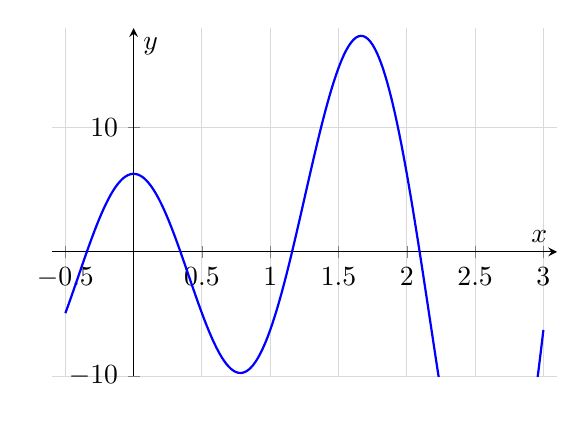
\begin{tikzpicture}
                \begin{axis}[
                    width=8cm,
                    height=6cm,
                    axis lines=middle,
                    xlabel=$x$,
                    ylabel=$y$,
                    xmin=-0.6,
                    xmax=3.1,
                    ymin=-10,
                    ymax=18,
                    grid=major,
                    grid style={gray!30},
                    samples=200,
                    domain=-0.5:3
                ]
                    \addplot[blue, thick] {-pi^2*x*sin(pi*x*180/pi)+2*pi*cos(pi*x*180/pi)};
                \end{axis}
            \end{tikzpicture}
        \end{image}
         \item Graph B:
        \begin{image}
            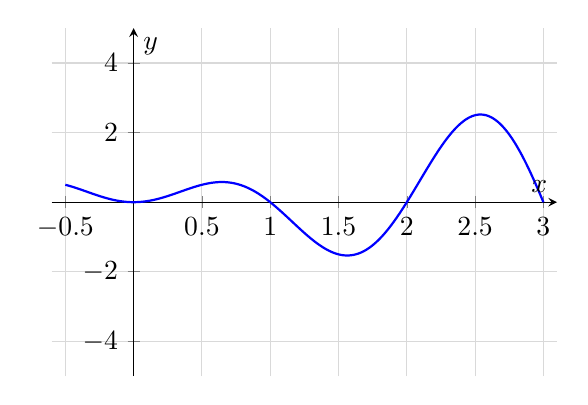
\begin{tikzpicture}
                \begin{axis}[
                    width=8cm,
                    height=6cm,
                    axis lines=middle,
                    xlabel=$x$,
                    ylabel=$y$,
                    xmin=-0.6,
                    xmax=3.1,
                    ymin=-5,
                    ymax=5,
                    grid=major,
                    grid style={gray!30},
                    samples=200,
                    domain=-0.5:3
                ]
                    \addplot[blue, thick] {x*sin(pi*x*180/pi)};
                \end{axis}
            \end{tikzpicture}
        \end{image}
        \item Graph C:
        \begin{image}
            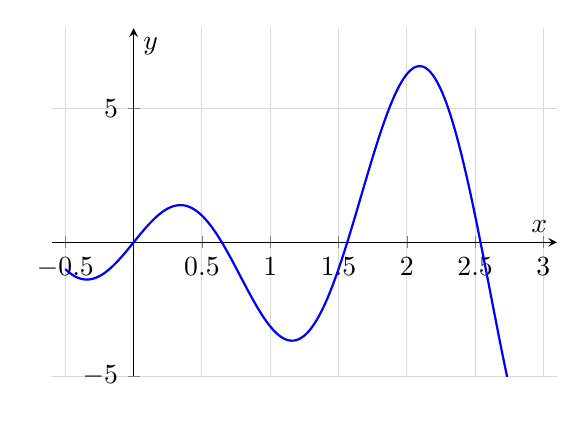
\begin{tikzpicture}
                \begin{axis}[
                    width=8cm,
                    height=6cm,
                    axis lines=middle,
                    xlabel=$x$,
                    ylabel=$y$,
                    xmin=-0.6,
                    xmax=3.1,
                    ymin=-5,
                    ymax=8,
                    grid=major,
                    grid style={gray!30},
                    samples=200,
                    domain=-0.5:3
                ]
                    \addplot[blue, thick] {pi*x*cos(pi*x*180/pi)+sin(pi*x*180/pi)};
                \end{axis}
            \end{tikzpicture}
        \end{image}
        
        \textcolor{blue}{The graph of each derivative should have zeros at each peak/valley of the original function.  It appears that (c) satisfies this for both (a) and (b).  Then, we can look at where the derivative of (a) and (b) would be positive.  The derivative of (a) should be negative before $x=0$, and then negative until about $x=2$, which (c) is not.  On the other hand, the derivative of (b) starts negative until $x=0$, then changes to positive until just after $x=2$, which is how (c) behaves.  Thus $f$ is (b) and $f'$ is (c).  This leaves (a) as $f''$. }
    \end{enumerate}

\end{exercise}


Problems adapted from Rogawski et al. \textit{Calculus: Early Transcendentals}, 4th Ed. 
\end{document}